\todoGeneric{10 à 15 pages de conception}

\section{Conception du robot}

\subsection{Conception mécanique}
\todoWho{Will}

Le lanceur de balles est une partie très importante du projet,
car il doit être capable de faire ce à quoi il est conçu de façon consistante pour faciliter son utilisation.
Il se sépare en 3 parties principales: la partie propulsion, la partie recharge ainsi que la partie visé.

\subsubsection{Mode de propulsion}
Pour la propulsion de la balle, trois systèmes ont été étudiés pour assurer une certaine précision tout en gardant le système simple.

\paragraph{Option 1 (par contact)}
Nous avons pensé à un système comprimant un ressort à l’aide d’une boîte de vitesse et d’une crémaillère.
Ce système à vite été écarté puisque nous ne savions pas si les pièces, principalement imprimées en PLA, allaient être capable de supporter l'énergie emmagasinée dans le ressort.
De plus, il aurait fallu avoir une façon de placer les balles à la bonne distance du ressort et les faire tenir en place avant le contact, ce qui aurait rapidement compliqué les choses.
Un solénoïde à aussi été envisagé pour frapper la balle, mais nos connaissance en magnétisme n’étaient pas adéquates pour considérer cette option plus sérieusement.

\todo{(Placer photo croquis)}

\paragraph{Option 2.1 (par piston)}
Un système comparable à ce que l’on retrouve dans les jouets de type “Airsoft” à aussi été étudié.
Ce système consiste encore une fois à comprimer un ressort attaché à un piston pour créer une différence de pression entre le devant et le derrière de la balle, la propulsant vers l’avant.
Ce système comporte les mêmes désavantages que la première option, en plus des problèmes d’étanchéité que peuvent apporter les pièces imprimées.
Il a donc été écarté.

\paragraph{Option 2.2 (par air comprimée)}
Nous avons pensé à remplacer le piston par une pompe à air et un réservoir pressurisé.
Sachant que l’air comprimé peut être très dangereux si le système échoue, et que nous allions être en présence de famille lors des démonstrations, cette option était donc une mauvaise idée.
De plus, un système comme celui-ci aurait été beaucoup plus compliqué que le système final choisi.
\todo{(Placer photo croquis)}

\paragraph{Option finale (roue d’inertie)}
Nous avons donc opté pour une roue d’inertie pour propulser nos balle.
L’idée est venue des jouets de la marque «NERF», qui utilisent 2 roues tournant en sens inverse pour propulser des fléchettes de mousse sur une distance acceptable.
Ce système est aussi assez simple, puisqu’il requiert seulement un moteur pouvant tourner à une vitesse contrôlable et d’une roue d’inertie.
Dans les lanceurs «NERF», les roues étaient en plastique dur, puisque que les projectiles étaient en mousse molle et très malléable.
Dans notre cas, nous ne voulions pas briser la balle, il a donc fallu rajouter une ruban extérieur en mousse servant à isoler les cadres de portes.

\todo{(Placer photo de la roue)}

\subsubsection{Méthode de chargement de la balle}
Quelques méthodes pour pousser les balles vers la roue d’inertie ont étés envisagées.
Voici les trois options principales.

\paragraph{Option 1 (par gravité)}
Nous avons pensé à utiliser la gravité pour pousser les balles sous la roue d’inertie pour simplifier le système.
Ce système aurait seulement eu besoin d’un servomoteur pour assurer qu’une seule balle tombe à la fois dans le lanceur.
Cependant, le système de roue d’inertie fait en sorte que la distance entre la roue et la base du lanceur est plus petit qu’une balle pour que la balle soit pressée dans la mousse et ainsi assurer un transfert d’énergie suffisant pour la propulser.
La gravité n’avait donc pas la force nécessaire pour enfoncer la balle sous la roue.

\paragraph{Option 2 (avec came et tige-poussoir)}
Nous voulions nous servir d’un servomoteur pour gérer le chargement, car ils sont simples à utiliser et assez précis pour nos besoins.
Le débattement nécessaire pour amener les balles de la position ou les balles sont placées jusqu’en dessous de la roue est d’environ 75 mm (les balles faisant 40mm de diamètre et en ajoutant quelques millimètres pour assurer la solidité du lanceur).
Les servos allant seulement de 0 à 180 degrés, il aurait fallu une camme d’au moins 75 mm de diamètre pour accommoder ce débattement, ce qui aurait été beaucoup trop gros en comparaison au lanceur.

\paragraph{Option 3 (avec pignon et crémaillère)}
Cet option est parfaite, puisqu’elle règle le seul problème que la came avait: la dimension des roues.
En se servant des CADs fournies par McMaster.com, il a été facile de trouver des pièces de dimensions adéquates pour notre système.
Un pignon ayant un diamètre primitif de 1 pouce ayant 20 dents et sa crémaillère répondaient parfaitement à nos critères de dimensions.
Il nous faudrait donc faire tourner le pignon une fois(2*pi*0,5 po) pour atteindre le débattement voulu (3po).
Il fallait donc changer 180 degrés du servo en 360 degré.
Nous avons donc utilisé deux roues ayant le même diamètre primitif que la première, dont une qui avait 2 fois plus de dents pour assurer un tour complet.
Les roues de 12 et 24 dents ont donc étés choisies, car elles etaient de bonnes dimensions.

\begin{figure}[h!]
    \centering
    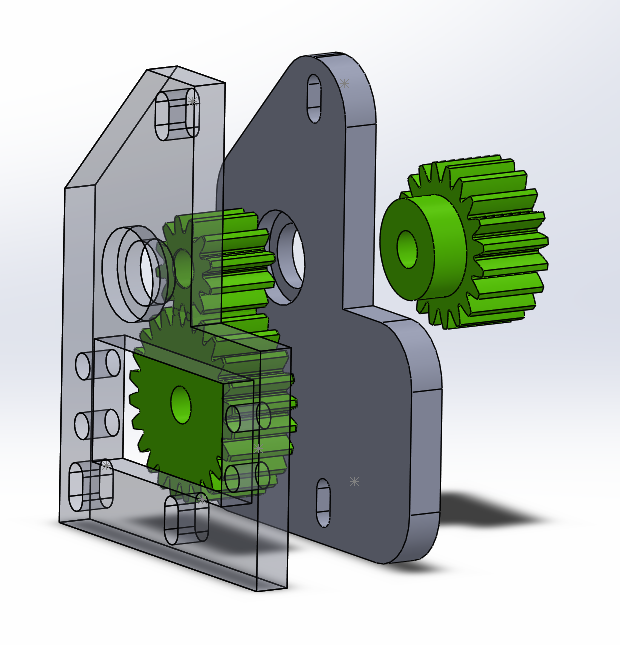
\includegraphics[width=0.5\linewidth]{img/s2/cad/gearbox1}
    \caption{Première itération de la boîte de vitesse}
    \label{fig:s2-cad-gearbox1}
\end{figure}

\subsubsection{Mode de visé}
Plusieurs options s’offraient à nous pour visé avec le lanceur.
La première étant de jouer avec l’angle du lanceur pour aller chercher différentes distances (pour atteindre tous les verres de beer pong).
Cette option a été écartée puisque nous ne savions pas le poids finale du lanceur et si un servomoteur allait être capable de le maintenir en place de façon constante.
Nous avons donc conçue un support ayant un arc de cercle ce qui nous a permit de choisir un angle et de sécuriser le lanceur à cet angle.

\begin{figure}[h!]
    \centering
    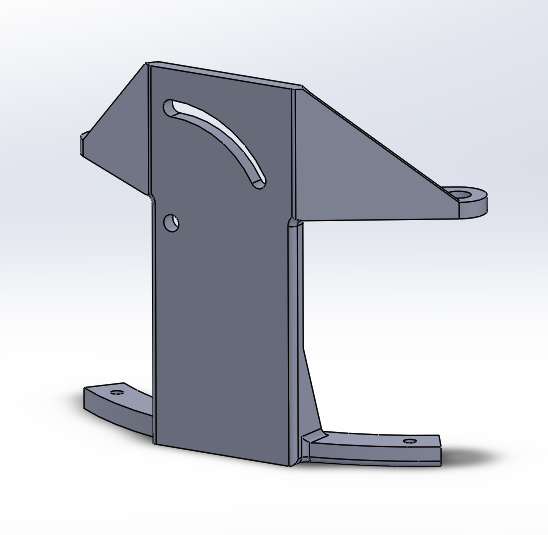
\includegraphics[width=0.5\linewidth]{img/s2/cad/support}
    \caption{Dernière itération du support à lanceur}
    \label{fig:s2-cad-support}
\end{figure}

La distance des lancers allait donc être déterminée par la vitesse à laquelle la roue d’inertie tourne, ainsi que la pression qu’elle applique sur les balles.

\subsubsection{Version finale du protype}
La version finale allait donc être un lanceur fixe rechargé par une crémaillère, qui propulse les balles à l’aide d’une roue d’inertie.
Notre première itération comportait une grande rampe pour assurer que les balles aient un maximum de temps en contact avec le lanceur pour augmenter la précision.
Cette idée de rampe a été abandonnée lorsque nous avons réalisé de quelle dimension elle devait être pour répondre à nos besoins (un arc de cercle d’environ 150 mm de rayon, pour assurer un arc de cercle assez graduel).
Nous avons donc optés pour un lancer direct avec un petit canon pour réduire les imprécisions des tirs.

\begin{figure}[h!]
    \centering

    \begin{subfigure}{0.3\linewidth}
        \centering
        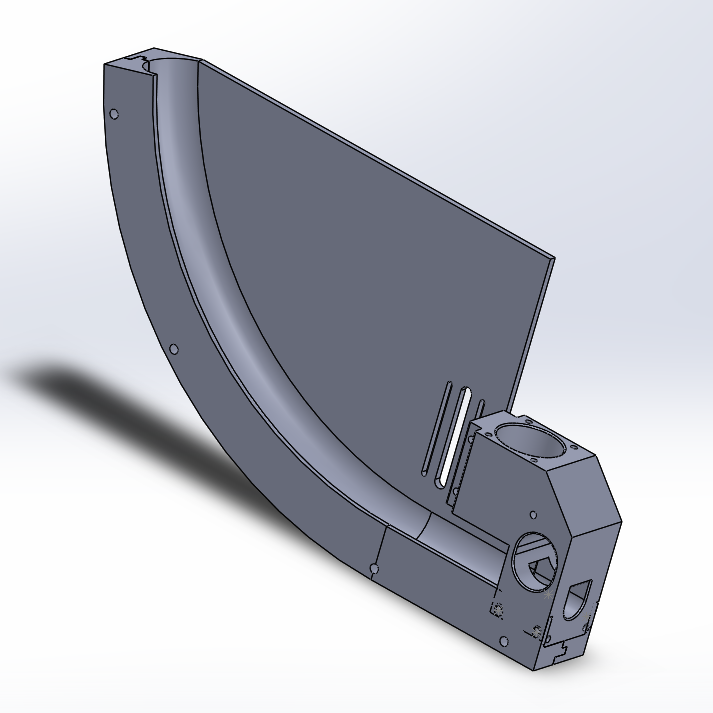
\includegraphics[width=\linewidth]{img/s2/cad/rampe}
        \caption{Modèle 3D de la rampe de lancement}
        \label{fig:s2-cad-rampe}
    \end{subfigure}
    \begin{subfigure}{0.3\linewidth}
        \centering
        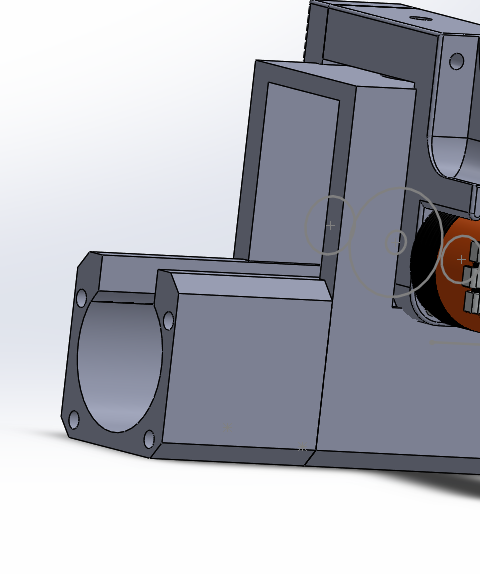
\includegraphics[width=\linewidth]{img/s2/cad/cannon}
        \caption{Modèle 3D du cannon}
        \label{fig:s2-cad-cannon}
    \end{subfigure}
    \caption{Rampe de lancement et cannon}
    \label{fig:template-example-flottante}
\end{figure}


Une autre amélioration de la version finale à été de fixer l’axe de la roue d’inertie des deux côtés et d’ajouter un roulement à bille.
Les pièces imprimées en 3D sont rarement balancées et la roue ajoutait beaucoup de vibration au système.
Le roulement à bille réduisait aussi la friction entre l’arbre de la roue et le support en plastique, qui avait tendance à fondre durant l’utilisation.
De plus, ce support facilitait aussi l’ajustement de la position de la roue d’inertie.
Un écrou sous le support était facilement accessible et nous n’avions plus besoins de défaire le montage au complet pour dévisser le moteur et changer sa hauteur.
Ce support était aussi imprimé en 2 pièces pour faciliter son implémentation au système.

\begin{figure}[h!]
    \centering
    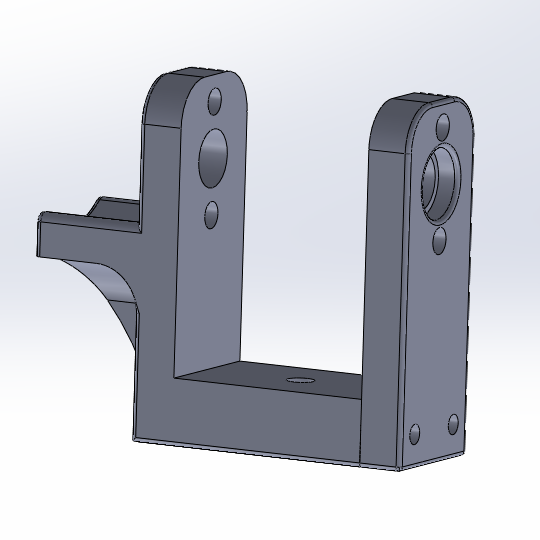
\includegraphics[width=0.5\linewidth]{img/s2/cad/motorholer}
    \caption{Modèle 3D du support à moteur}
    \label{fig:s2-cad-motorholer}
\end{figure}

\todo{ajouter photo dans image.zip}

Pour assurer un maillage adéquat entre les roues de la boîte de transmission et la crémaillère, des trous oblongs avaient étés utilisés.
Cependant, nous nous sommes rendu compte que ces trous ne servaient pas à grand chose et que les engrenages devaient être plus contraintes.
La position du servomoteur a aussi été modifiée puisqu’il interférait avec les tiges filetées servant à fixer le système.
Nous avons donc conçue une boîte de transmission complètement indépendante du lanceur qui gardait toujours la bonne distance entre les engrenages.
Cette boite était par la suite fixée au lanceur à l’aide des trous prévus à cette effet.

\begin{figure}[h!]
    \centering
    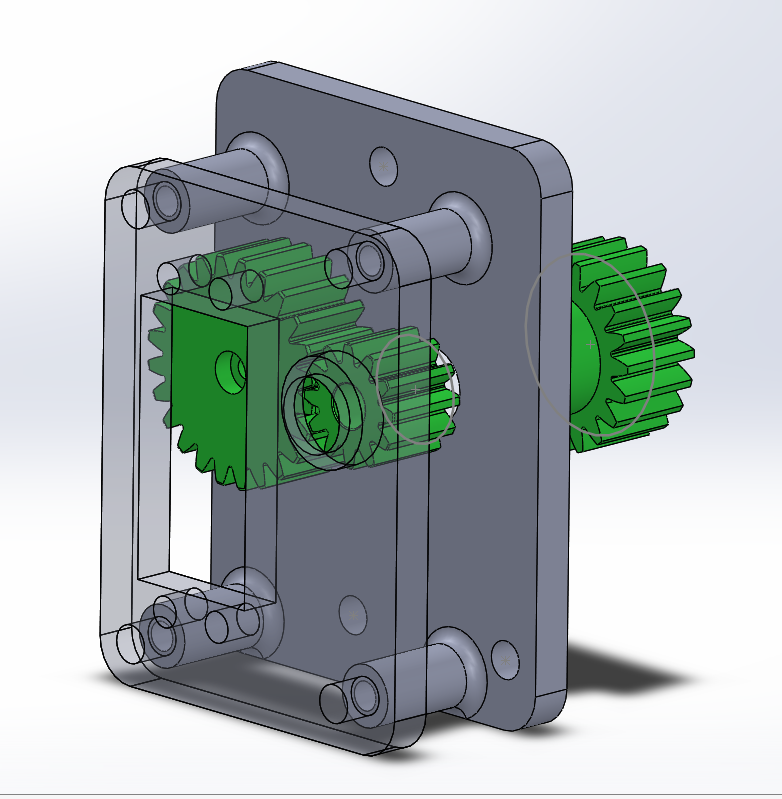
\includegraphics[width=0.5\linewidth]{img/s2/cad/gearbox2}
    \caption{Dernière itération de la boîte de vitesse}
    \label{fig:s2-cad-gearbox2}
\end{figure}


\todo{ajouter photo}
Le PLA est un plastique malléable et facile à percer.
Nous nous sommes servis de ces caractéristique pour décortiquer notre lanceur en pièces faciles à imprimer et nous avons utilisés des tiges filetées de dimensions 10-32 pour tenir le tout ensemble.

\begin{figure}[h!]
    \centering

    \begin{subfigure}{0.4\linewidth}
        \centering
        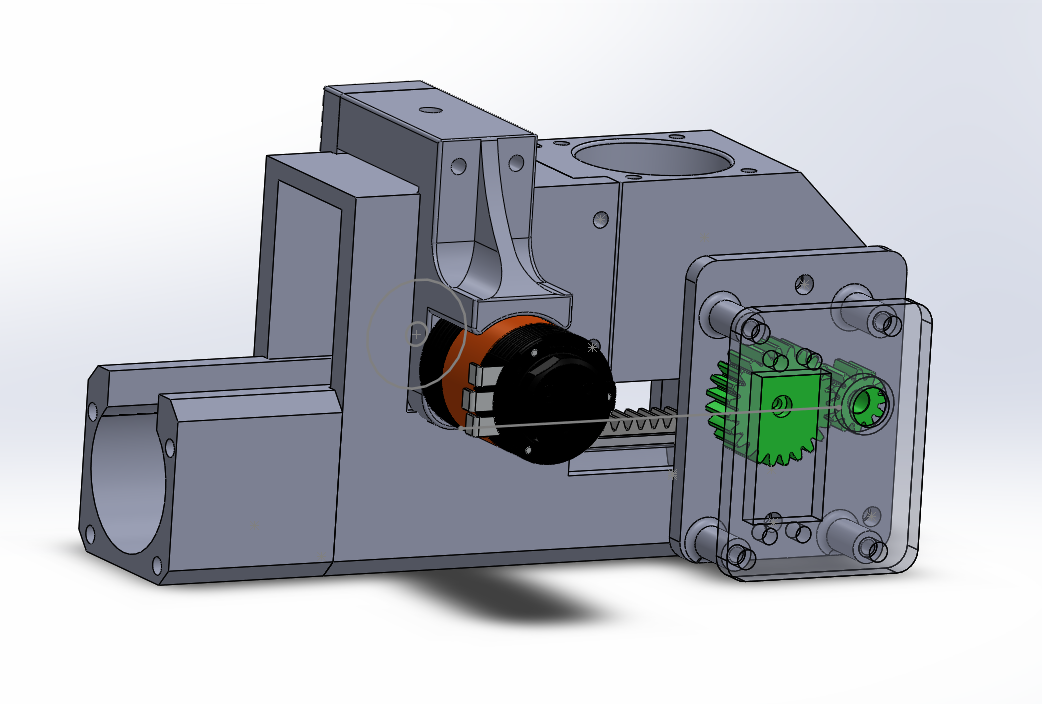
\includegraphics[width=\linewidth]{img/s2/cad/lanceur1}
        \caption{Vue d'ensemble du premier lanceur}
        \label{fig:a1-s2-cad-lanceur1}
    \end{subfigure}
    \begin{subfigure}{0.4\linewidth}
        \centering
        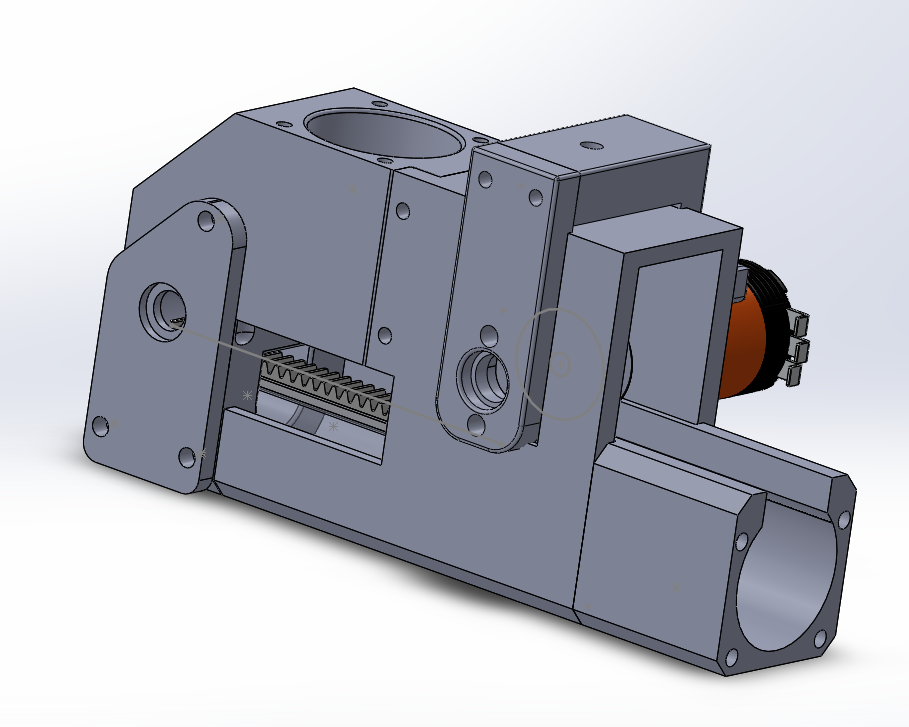
\includegraphics[width=\linewidth]{img/s2/cad/lanceur2}
        \caption{Vue d'ensemble du lanceur final}
        \label{fig:a1-s2-cad-lanceur2}
    \end{subfigure}

    \caption{Description de l'image.}
    \label{fig:template-example-flottante}
\end{figure}


\todo{ajouter photo prises par mathieu du lanceur monter}

\subsection{Conception électronique}
\todoWho{Jordan}

Puisque la méthode de lancer choisi est la roue d’inertie et la méthode de chargement est avec un pignon et une crémaillère, nous devions intégrer au montage un moteur DC et un servomoteur.
Ainsi le moteur choisi pour faire tourner la roue d’inertie servant à propulser la balle est un moteur DC sans balai.
Nous avons opté pour ce type de moteur puisque le nombre de rotation par minute devait être suffisamment élevé pour propulser la balle assez loin et le torque devait également être suffisamment important pour éviter une obstruction lors du passage de la balle.
L’un d’entre nous possédait un moteur pouvant servir au projet, c’est donc lui qu’on a utilisé.
Il s’agit du moteur TrackStar 8.5T.

\todo[inline]{add image}

Puisque c’est un moteur sans balai, il ne suffit pas seulement d’appliquer une tension à ses bornes pour qu’il tourne.
Nous avons donc acheté un contrôleur servant à faire tourner le moteur et à modifier la vitesse grâce à un signal d'entrée.
Le contrôleur choisi est le ESC 30A.
Ce contrôleur a comme entrées une alimentation qui doit être d’environ 7,4~V pour que le moteur fonctionne comme il se doit selon la fiche technique du moteur \cite{noauthor_trackstar_nodate} et trois autres fils qui doivent être branché sur l’Arduino.
Ces trois fils doivent être branché au commun de l’Arduino, au 5~V et à une sortie pouvant produire un PWM soient les broches 2 à 13 de l’Arduino Mega.
Les trois fils de sorties du contrôleur sont branchés directement sur les trois fils du moteur.
Pour ce branchement, il a été très important de vérifier que le commun de l’alimentation soit connecté au commun de l’Arduino.

\todo[inline]{add image: Circuit d'alimentation et de contrôle du moteur DC sans balai}

Par ailleurs, le moteur doit recevoir une tension d’alimentation de 7,4~V comme indiqué sur la figure\todo{make ref to figure}.
Cependant, les seules prises d’alimentation sur le robot pouvant fournir un gros courant sont des prises de 5~V et 12~V.
Ainsi, nous avons acheté un régulateur de tension de type buck pour pouvoir passer de 12~V à 7,4~V.
Le régulateur de tension acheté est le VMA404 utilisant un LM2596, car c’était un modèle peu dispendieux disponible à la boutique Electro5 de Sherbrooke.
Comme indiqué dans la prochaine figure\todo{Add ref to figure}, la tension d’entrée est de 12~V et en mesurant la tension de sortie avec un multimètre nous pouvons ajuster le potentiomètre pour avoir 7,4~V en sortie.

\todo[inline]{add image: Régulateur de tension VMA404}

Pour ce qui est du servomoteur, ce dernier est branché directement dans l’un des ports d’entrée sur la carte Robus conçu à cet effet.

Ensuite, pour la communication Bluetooth, nous avons acheté le module HC-05, car c’était celui qui avait était suggéré par le technicien Serge lors du séminaire sur les capteurs.
Son branchement est effectué comme à la prochaine figure\todo{Add ref to figure}.

\todo[inline]{add image: Circuit de branchement du module Bluetooth HC-05}

On voit donc sur la figure \todo{Add ref to figure} que le module a 4 fils de branchement.
Il y a deux fils pour l’alimentation, et deux fils pour la réception et la transmission du signal.
Le module marche à des tensions de 3,3~V, c’est pourquoi il y a le diviseur de tension à l’entrée RXD du module comme suggéré sur le site \cite{noauthor_setting_nodate}.
L’alimentation est toutefois branchée au 5~V, car il y a un régulateur interne sur le module Bluetooth pour passer de 5~V à 3,3~V.

\subsection{Conception logiciel}
\todoWho{Thierry}

\todo[inline]{add pseudocode}

\todo[inline]{add Diagramme d’activité}

La programmation du robot peut sembler compliqué, mais en réalité elle était très simple.
L’application Android, qui est conçue pour communiquer avec le robot, envoie un chiffre en fonction de l’action que veut faire l’utilisateur.
Par exemple, si l’utilisateurs appuie sur la balle pour tirer, le téléphone va communiquer avec le récepteur Bluetooth du robot en lui envoyant le chiffre 6.

\todo[inline]{add image}

Le chiffre envoyé est de type «char».
Pour simplifier la compréhension du code, nous avons initialisé chacune des constantes et avons attribué une variable représentative.
La \todo{insert reference (maybe figure)} représente chacune des constantes qui ont été initialisé.
Ensuite, lors de la configuration de l'Arduino, le Bluetooth est initialisé avec les broches correspondantes.
De plus, le moteur sans balai que nous avons utilisé est configuré comme un servomoteur, donc nous avons utilisé la classe MegaServo pour initialiser ce moteur.
Les valeurs à rentrer en paramètre de la fonction ne sont pas des angles puisque c’est un moteur sans balais.
Selon \cite{arduino_arduino_2019} le contrôleur du moteur reçoit une impulsion entre 1000~$\mu$s et 2000~$\mu$s, c’est pourquoi nous utilisons ces valeurs.
Dans ce cas, 1000 représente la valeur minimum c’est-à-dire que le moteur ne tourne pas, alors qu’à 2000, le moteur tourne à sa pleine capacité.
Le servo moteur a été configurer avec la libraire LibRobus, qui nous a été offerte.

La boucle vérifie à chaque fois si l’application a envoyé un message.
Lorsqu’un message est reçu, l’Arduino exécute l’action demandé.
L’action d’avancer et de reculer est très simple, elle consiste uniquement à configurer les 2 moteurs à 0,2~V pour avancer et à -0,2~V pour reculer.
Nous avons jugé que l’utilisation du PID pour cette fonction n’était pas nécessaire, puisque le robot ne fait que de très petits mouvements.
Ensuite, lorsque l’utilisateur relâche le bouton, un second message est envoyé au robot pour configurer les 2 moteurs à 0~V (les arrêter).

Les trois prochaines conditions sont reliées au canon du robot.
Lorsque l’utilisateurs demande un incrément de la vitesse du moteur, la variable forceMoteur est incrémentée de 5.
Pour la condition où le joueur demande une décrémentation, la vitesse du moteur est décrémentée par 5.
Pour la distance que nous désirions des verres, après quelques tests, nous avons réalisé que la vitesse optimale était entre 1150 et 1200.
C’est pourquoi les 10 niveaux de forces du moteur se situent entre 1150 et 1200.
Ensuite, lorsque le joueur appuie sur «tirer», l’Arduino reçoit comme commande de tirer.
L’angle du servomoteur est donc configurer pour reculer à son minimum, et retourner à son angle initial de 180 degrés.
Durant cette action, le moteur sans balai part sa puissance à la vitesse demandée par l’utilisateur.
Donc, lorsque la balle est poussée dans la roue de mousse reliée au moteur sans balai, la balle est propulsée et l’Arduino envoie comme message de fermé le moteur DC.
Au départ, nous voulions laisser le moteur sans balai rouler en tout temps, cependant par souci d’économie d’énergie et pour que le système soutenant le moteur s’use moins rapidement, nous avons décidé de le partir uniquement lorsque l’Arduino reçoit la commande de tirer.

\subsection{Conception logiciel de l'application}
\todoWho{Thierry}

C’était la première fois que nous programmions une application Android, c’est pourquoi nous avons choisi d’utiliser Mit App Inventor.
Cette plateforme est une façon très simple de programmer une application sans pour autant devoir apprendre un nouveau langage de code.
Une autre des raisons que nous avons choisi d’utiliser cette application est la facilité avec la communication Bluetooth.
Tout était déjà intégré dans l’application, il manquait uniquement à associer chacun des boutons avec le message que l’on voulait envoyer.
Comme mentionné dans la section du robot, le message envoyé est de type «char».
Nous avons choisi d’envoyer cela au lieu d’une chaine de caractère puisqu’il était plus facile de manipuler les caractères.

\section{Conception du système de verres}

Le système de verres est ce qui reçoit les balles lancées par le lanceur de balles.
C’est un système composé d’un plateau où sont déposés six verres.
Dans chacun de ces verres, il y a un capteur détectant la présence d’une balle ou non.
Dans ce projet, tous les schémas électriques du système de verres sont faits avec le logiciel \emph{KiCad} et la conception mécanique est faite avec le logiciel \emph{SolidWorks}.

\subsection{Conception mécanique}
\todoWho{Vincent}

La partie mécanique du système de verre comprend la conception du plateau ainsi que tout ce qu’il y est fixé, soit les verres, le boitier électrique ainsi que le toit.
Le plateau est composé d’une base carrée en bois dont les côtés ont quatorze pouces et demi de longueur.
Sur chaque côté de la base, il y a des bordures de deux pouces demis de haut par trois-quarts de pouce de largeur.
Il y a également six verres fixés sur la base formant un triangle.
Ensuite, sur trois des quatre bordures il y a des supports où est déposé le toit du plateau.
Celui-ci est fait en mélamine et il comporte six troues de quatre pouces de diamètre alignés avec les verres.\todo{add citation}
Finalement, le boitier électrique est fixé sur l’extérieur de la bordure droite de 3 pouces.
L’image \todo{add ref to figure} ci-dessous illustre l’allure finale du plateau de verres.

\todo[inline]{add image: Plateau de verres}

Pour être en mesure de bien effectuer sa conception, il a fallu répondre à certaines contraintes.
Celles-ci sont que le plateau doit avoir une belle esthétique tout en étant assez gros pour contenir six verres et assez petit pour être en mesure de le déplacer et de le ranger facilement.
Il doit aussi être fait de façon à rendre accessible tout ce qui est d’électronique à l’intérieur.
De plus, le coût de réalisation ne devait pas être trop élevé vu le statut d’étudiant des membres de l’équipe.

La base ainsi que les bordures du plateau auraient pu être imprimées à partir d’une imprimante 3D, mais les dimensions sont très grandes rendant le coût de son impression très élevé dû au prix du plastique ABS.
Aussi, l’utilisation de ce type d’imprimante n’est pas justifiée dû au fait que le plateau comporte peu de détailles.
Ensuite, parce que son coût est très faible, le bois a été choisi pour le matériau du plateau.
Les bordures ainsi que la base sont fixées ensemble par de la colle à bois en plus de clous de finissions.
Le choix de la mélamine comme matériau pour le toit s’explique par le fait qu’il est beaucoup plus mince que le bois en général.
Vu que le toit s’enlève pour la maintenance du plateau, son épaisseur est importante pour que sa manipulation soit plus facile.
La fixation des verres dans la base est nécessaire, car pour être en mesure de bien détecter une balle, les capteurs installés sur le côté des verres se doivent d’être immobiles.

\subsection{Conception électrique}
\todoWho{Vincent}

La conception électrique du système de verres est faite en quatre parties.
La première est le circuit d’alimentation du système, la deuxième est la conception du capteur qui détecte les balles dans les verres, la troisième est la conception du circuit permettant la gestion du signal d’entrée du capteur à l'Arduino et la quatrième partie est le circuit effectuant la gestion du signal sortie provenant de l’Arduino.

\subsubsection{Alimentation}

L’alimentation électrique du système de verres se fait à 9~V, car il s’agit du standard pour ce type de circuit électronique.
Le circuit d’alimentation est illustré dans les figures ci-dessous\todo{add ref to figure}.

\todo[inline]{add figures:Circuit d’alimentation 9~V et Alimentation Arduino mega2560 R3}

L’alimentation 9~V provient de deux piles 9~V alimentant chacune deux parties différentes du système.
Dans la figure 1\todo{add ref to figure}, elles se nomment 9V-1 et 9V-2.
La première alimentation alimente tous les circuits électriques du plateau de verres et la deuxième alimente l’Arduino.
De plus, chacune des bornes négatives est connectée ensemble pour que le circuit aille le même commun.
Les interrupteurs présentent dans le circuit de la figure ont comme fonction de faire commuter la tension des piles vers leurs circuits respectifs.
Les diodes électroluminescentes vertes (DEL) servent de témoins lumineux indiquant l’état des circuits du plateau ainsi que de l’Arduino.
Ces DEL sont chacune en série avec une résistance limitant le courant traversant les DEL à 10,3~mA, car la différence de potentiel aux bornes de ce type de DEL varie autour de 2~V normalement.\todo{add citation}
Il est préférable d’utiliser deux piles plutôt qu’une pour augmenter la durée de vie des batteries.
Ce circuit se situe dans le boitier électrique.

\subsubsection{Capteurs}

Les capteurs sont la partie centrale du système de verre.
Leurs circuits sont alimentés à 9~V et sont composés d’une DEL à rayonnement infrarouge pointée vers une photodiode filtrée pour ne laisser passer que les rayons infrarouges.
Ce circuit est illustré schématiquement par la figure ci-dessous \todo{add ref to figure} et il est monté sur une plaquette de prototypage située à l’intérieur du plateau de verres.

\todo[inline]{add figures: Circuit du capteur}

Dans le circuit de la figure 2\todo{add ref to figure}, les DEL infrarouges sont représentées par IR\_D et les photodiodes par PD.
Ces deux composants sont installés sur chacun des verres un en face de l’autre.
Pour ce qui est de la DEL infrarouge, vu que la différence de potentiel à ses bornes varie typiquement autour de 1,2~V, une résistance de 430~$\omega$ est nécessaire dans le but de limiter le courant y circulant à 18~mA.
\todo{add citation}
Pour ce qui est de la photodiode, elle est branchée en sens contraire de sorte que la cathode soit connectée à l’alimentation positive du circuit.
\todo{add citation}
L’utilisation d’une DEL infrarouge comme émetteur plutôt que toute autre DEL est due au fait que son rayonnement est invisible à l'oeil nu.
La photodiode est choisie pour capter les rayons infrarouges, car elle réagit très fortement à une faible variation de rayon la traversant.
Cette caractéristique est très importants dû au fait que c’est une balle de ping-pong qui coupe les rayons dans le verre.
Même si ce n’est pas ce qui est de meilleur pour couper effectivement les rayons infrarouges, la balle réussie quand même à couper une partie des rayons et la photodiode sera plus sensible à ce faible changement qu’un phototransistor par exemple.

\subsubsection{Modulation du signal d’entrée}

Le fonctionnement d’une photodiode se fait en laissant passer un courant maximum en 35~$\mu$A en sens inverse lorsqu’elle est illuminée par la DEL infrarouge.\todo{add citation}
Ce courant se transforme éventuellement en signal d’entrée pour le microcontrôleur.
Ce circuit est illustré sur la figure ci-dessous.\todo{add ref to fig}
\todo{add citation}

\todo[inline]{add figures: Circuit modulant signal d’entrée}

Dans la figure 5\todo{add refto figure}, ce qui fait la transformation du signal provenant des capteurs en signal d’entrée digital pour l’Arduino est six amplificateurs opérationnels (ampli-op) MPC602 agissant en comparateur, soit un par verre.
Ceux-ci laissent soit passer 0~V, lorsqu’il n’y a pas de balle dans un des verres, ou 5~V lorsqu’une balle vient couper les rayons infrarouges.
\todo{add citation}
Pour se faire, le signal provenant du capteur doit se connecter à la borne (-) de l’ampli-op et la tension de référence (Vref) à la borne (+).
Aussi, pour être compatible avec l’Arduino, l’amplificateur opérationnel doit donner en sortie une tension de 5~V.
\todo{add citation}
Les ampli-op doivent donc être alimentés à 5~V.
Le composant faisant passer la tension d’alimentation 9V-2 à 5~V est un régulateur de tension 5~V LM7805.
\todo{add citation}
Vu que la tension à l’entrée (+) de l’ampli-op est presque nulle, la tension de référence Vref posée est de 0,5~V.
Cette tension est créée par un diviseur de tension alimenté à 5~V comprenant une résistance de 91~k$\omega$ et 10~k$\omega$.
Pour que le courant provenant de la photodiode se transforme en signal d'entré, celui-ci doit passer à travers une résistance de 150~k$\omega$ pour qu’il y aille une tension de 5~V à ses bornes si le courant la traversant est de 35~$\mu$A lorsque les rayons infrarouges ne sont pas coupés.
En réalité, la tension à ses bornes varie entre 0,65~V à 1,2~V selon chaque verre dû à l’enlignement des diodes infrarouges avec les photodiodes.
De plus, lorsqu’une balle coupe les rayons, la tension s’abaisse à une valeur variante entre 0,2~V à 0,4~V selon chaque verre.
Dans chacun des cas, les tensions aux bornes des résistances sont cohérentes par rapport à Vref.

Dans ce dernier circuit, il était préférable d’utiliser un ampli-op agissant en comparateur au lieu d’un vrai comparateur dû au fait que la sortie de l’ampli-op est tant en PNP qu'en NPN tandis que la sortie du comparateur est seulement NPN.
\todo{add citation}
En effet, vu que la sortie de l’amplificateur se connecte directement l’Arduino, il est préférable d’utiliser un composant PNP, car celui-ci ne nécessite pas l’ajout d’une résistance en amont de la sortie permettant au courant de circuler.
Pour ce qui est des régulateurs de tension LM7805, leurs utilisations sont justifiées par le fait que ce type de composant n’est pas affecté par le courant circulant dans les amplificateurs et ils régulent la tension qu’ils reçoivent en entrée, peu importe sa valeur pourvu qu’elle soit supérieure à 7~V, car celui-ci comporte une perte de deux volts.
\todo{add citation}
Finalement, dans le circuit de la figure 3\todo{add ref to figure}, les condensateurs C1 et C2 sont nécessaires, car ils diminuent le bruit dans le circuit.
Ce circuit est monté sur une plaquette de prototypage se situant à l’intérieur du boitier électrique noir.

\subsubsection{Signal de sortie}

La dernière partie de la conception est celle contrôlant le signal du circuit de sortie.
Ainsi, lorsque l’Arduino ne reçoit plus 5~V en entrée d’un des verres, celui-ci envoie un signal de 5~V dont le but sera d’alimenter une des DEL bleues se trouvant sur le toit du plateau.
Le circuit de ces DEL est présenté sur la figure 6\todo{add ref to figure}.

\todo[inline]{add figures: Circuit de sortie du Arduino}

Sur la figure 4\todo{add ref to figure} ci-dessus, il y a une résistance de 390~$\omega$ en série avec chacune des DEL, car la tension aux bornes de ce type de DEL varie typiquement autour de 3,2~V.
\todo{ass citation}
Ainsi, ces résistances limitent le courant circulant dans les DEL à environ 4,6~mA.
Les DEL de couleurs bleues ont été choisies tout simplement parce qu’elles sont belles et qu’elles brillent bien de façon générale.
Elles agissent comme témoins lumineux lorsque l’Arduino détecte qu’il y a une balle dans un des verres.
Ce circuit est également monté sur la plaquette de prototypage du boitier électrique.

\subsection{Conception logiciel}
\todoWho{Thierry}

\todo[inline]{add pseudocode}

\todo[inline]{add Diagramme d’activité}

Pour les verres, il fallait programmer l'Arduino Mega 2560 qui a été utilisé.
Cette programmation était relativement simple.
Six des entrées digitales (configurées en entrées) de l'Arduino étaient connectées aux verres, ces entrées sont les broches 22 à 32.
Ces entrées sont par incrément de 2, ce qui totalise les six verres.
Six autres entrées digitales (configurées en sortie) étaient connectées aux DEL, ceux-ci sont les entrées 1 à 7.
Lors de la configuration de l'Arduino (init), une tension de cinq volts par sorties digitales est envoyé pour allumer les DEL.
Ensuite, le programme passe à la boucle.
La boucle (loop) vérifie si une balles est entrée dans les verres.
Le programme sait lorsqu'un verre est réussi en vérifiant les entrées digitales 22 à 32.
Lorsque l'entrée ne détecte plus une tension de 5 V, un message est envoyé pour fermer la DEL correspondante.
Les DEL ont été organisées pour que chaque sortie corresponde au bon verre.
Par exemple, la DEL 22 est reliée à l’entrée 1, la DEL 24 est reliée à l’entrée 2 etc.
